% Created 2024-02-19 ma 09:14
% Intended LaTeX compiler: pdflatex
\documentclass[bigger]{beamer}
\usepackage[utf8]{inputenc}
\usepackage[T1]{fontenc}
\usepackage{graphicx}
\usepackage{longtable}
\usepackage{wrapfig}
\usepackage{rotating}
\usepackage[normalem]{ulem}
\usepackage{amsmath}
\usepackage{amssymb}
\usepackage{capt-of}
\usepackage{hyperref}
\usepackage{graphicx}
\usepackage[export]{adjustbox}
\usetheme{default}
\author{Jeroen van Riel}
\date{February 2024}
\title{Trajectory Planning}
\hypersetup{
 pdfauthor={Jeroen van Riel},
 pdftitle={Trajectory Planning},
 pdfkeywords={},
 pdfsubject={},
 pdfcreator={Emacs}, 
 pdflang={English}}
\usepackage{natbib}
\begin{document}

\maketitle
\begin{frame}[label={sec:org2c0fe4f}]{Offline crossing time scheduling}
\vfill
\begin{figure}
  \centering
  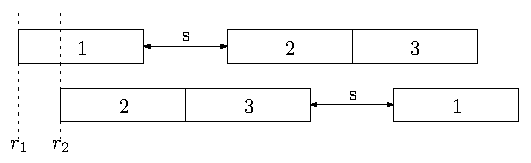
\includegraphics[width=0.6\textwidth]{figures/123.pdf}
\end{figure}

\begin{itemize}
\item given schedule \(y\), there always exist trajectories \(x\) that are \emph{safe}
\item solve a MILP to obtain optimal \(y\)
\item heuristic methods
\begin{itemize}
\item polling policies such as exhaustive, gated or k-limited
\item \emph{learning} method such as RL
\end{itemize}
\end{itemize}
\end{frame}
\begin{frame}[label={sec:org7e2b44e}]{Online trajectory planning (Miculescu \& Karaman)}
\begin{itemize}
\item recalculate trajectories upon new arrivals
\item \emph{regular} polling policy
\item MotionSynthesize produces \emph{safe} trajectories
\end{itemize}

\begin{figure}
  \centering
  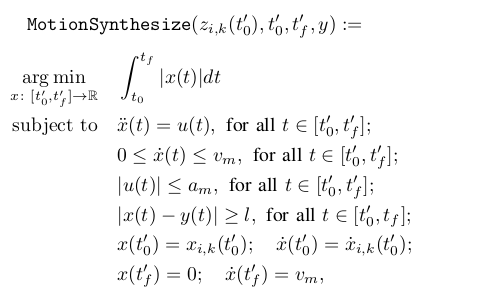
\includegraphics[width=0.6\textwidth]{figures/MotionSynthesize.png}
\end{figure}
\end{frame}
\begin{frame}[label={sec:org8eb72e4}]{Offline crossing time scheduling in network}
\begin{itemize}
\item problem like classical job-shop
\item solve as MILP
\item heuristic methods
\begin{itemize}
\item Zhang et al. train an RL agent to constructs a job-shop schedule by
adding/removing arcs to the corresponding disjunctive arc
\item their method might also work in an online setting
\end{itemize}
\end{itemize}
\end{frame}
\begin{frame}[label={sec:orgb48ad04}]{Trajectory planning in network}
\begin{itemize}
\item need to consider finite space between intersection
\item finite buffers can be modeled in the MILP (under some assumptions on vehicle routes)

\vfill
\item it is not clear that safe trajectories always exist for some crossing time
schedule \(y\), as was shown for the single intersection case
\end{itemize}
\end{frame}
\begin{frame}[label={sec:orgaebe8b7}]{Online trajectory planning in network}
\begin{itemize}
\item generate trajectories based on a crossing time schedule

\vfill
\item alternatively, the control problem can be stated directly in terms of
(approximations of) trajectories
\begin{itemize}
\item idea: determine the waiting time on fixed \emph{locations}
\end{itemize}
\end{itemize}

\begin{figure}
  \centering
  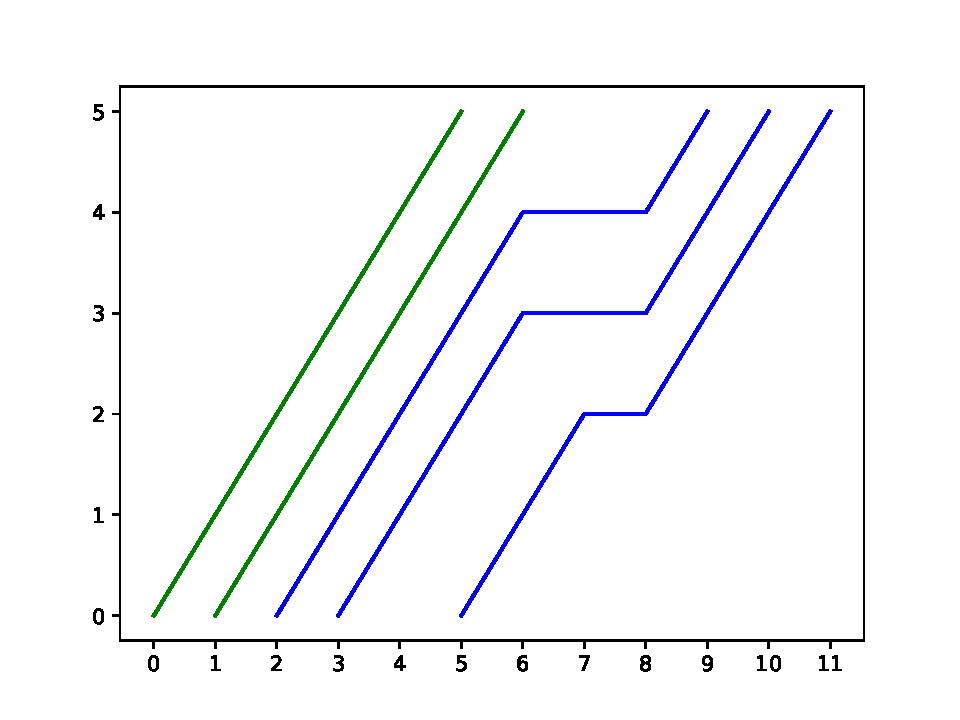
\includegraphics[width=0.6\textwidth]{figures/finite-buffer-schedule.pdf}
\end{figure}
\end{frame}
\end{document}
